%!TEX root = /Users/stevenmartell/Documents/CURRENT PROJECTS/iSCAM-trunk/docs/iSCAM-guide/overView.tex
\section{Installation} % (fold)
\label{sec:installation}


\subsection[Source code]{Obtaining source code} % (fold)
\label{sub:obtaining_source_code}

\begin{frame}[containsverbatim]
	\frametitle{Obtaining \iscam\ source code}
	Source code available at:\\
	\url{http://code.google.com/p/iscam-project/}
	\vfill
	Use subversion to checkout a copy
	\vfill
	\underline{On Mac \& Linux, in Terminal:}
	\tiny
	\begin{verbatim}
		svn checkout http://iscam-project.googlecode.com/svn/trunk/			iscam-project-read-only
	\end{verbatim}
	\normalsize
	\vfill
	\underline{On Windows use a subversion client}
	\url{http://tortoisesvn.net/}
\end{frame}

% subsection obtaining_source_code (end)
\subsection{SVN commands} % (fold)
\label{sub:svn_commands}
\begin{frame}
	\frametitle{Useful SVN commands}
	Usage: \texttt{svn command}
	\vfill
	\begin{scriptsize}
	\begin{tabular}{ll}
		Command & Description\\
		\hline
		\texttt{checkout} & Check out a working copy from a repository.\\
		\texttt{info}     & Display information about a local or remote item.\\
		\texttt{update}   & Bring changes from the repository into the working copy.\\
		\texttt{log}      & Show the log messages for a set of revision(s) and/or file(s).\\
		\texttt{revert}   & Restore pristine working copy file (undo most local edits).\\
		\texttt{commit}   & Send changes from your working copy to the repository.\\
		\texttt{diff}     & Display the differences between two revisions or paths.\\
		\texttt{help}     & Display help (usage \texttt{svn help <command>})\\
		\hline
	\end{tabular}
	\end{scriptsize}
\end{frame}
% subsection svn_commands (end)

\subsection{Directories} % (fold)
\label{sub:directories}
\begin{frame}
	\frametitle{Directory structure}
	\begin{columns}
	%
	\begin{column}{2in}
	\texttt{
	\begin{itemize}
		\item iSCAM-trunk
		\begin{itemize}
			\item dist
			\only<2>{
			\begin{itemize}
				\item debug
				\item R
				\item release
			\end{itemize}
			}
			\item docs
			\only<3>{
			\begin{itemize}
				\item API
				\item iSCAM-guide
				\item userGuide
			\end{itemize}
			}
			\item examples
			\only<4>{
			\begin{itemize}
				\item 4VWXHerring
				\item Cusk
				\item ...
				\item Makefile
				\item makeproject
			\end{itemize}
			}
			\item fba
			\only<5>{
			\begin{itemize}
				\item BC-herring-2011
				\item makeproject
				\item ReadMe.txt
			\end{itemize}
			}
			\item scripts
			\only<6>{
			\begin{itemize}
				\item scripts
			\end{itemize}
			}
			\item src
			\only<7>{
			\begin{itemize}
				\item admb-code
				\item r-code
			\end{itemize}
			}
		\end{itemize}
	\end{itemize}
	}
	\end{column}
	
	\begin{column}{2in}
		\only<2>{\texttt{dist} contains the compiled ADMB code
		 in debug and release versions, and the R scripts for 
		 dealing with output.}
		
		\only<3>{\texttt{docs} contains directories for the users
		guide, this presentation, and the API documentation for 
		the source code.\\[1ex]
		
		The users guide and presentation is written in latex, and 
		the API is built using doxygen.}
		
		\only<4>{\texttt{examples} directory contains several different
		examples and a Makefile for running the examples. \\[1ex]
		\texttt{makeproject}
		is a Unix script for setting up a new example directory.}
		
		\only<5>{\texttt{fba} is a directory for ``full blown assessment''\\[1ex]
		The ReadMe.txt file documents the various projects, and  \texttt{makeproject}
		is a Unix script for setting up a new assessment directory. }
		
		\only<6>{\texttt{scripts} contains various scripts that are copied into
		assessment directories. }
		
		\only<7>{\texttt{src} contains directories for the ADMB source code and the R-code and source files for the R-package.}
	\end{column}
	%
	\end{columns}
\end{frame}
% subsection directories (end)

\subsection{Text Editors} % (fold)
\label{sub:text_editors}


\begin{frame}
	\frametitle{Editors}
	\only<1>{
	\underline{Windows}
	\begin{itemize}
		\item Textpad \url{http://www.textpad.com/}
	\end{itemize}
	\underline{Mac OSX}
	\begin{itemize}
		\item Textmate \url{http://macromates.com/}
	\end{itemize}
	\underline{Linux}
	\begin{itemize}
		\item Vim \url{http://www.vim.org/}
	\end{itemize}
	\underline{Cross platform}
	\begin{itemize}
		\item Emacs \url{http://www.gnu.org/s/emacs/}
		\item eclipse \url{http://www.eclipse.org/}
		\item sublime \url{http://www.sublimetext.com/}
	\end{itemize}
	}
	\only<2>{
	\begin{figure}[htbp]
		\centering
			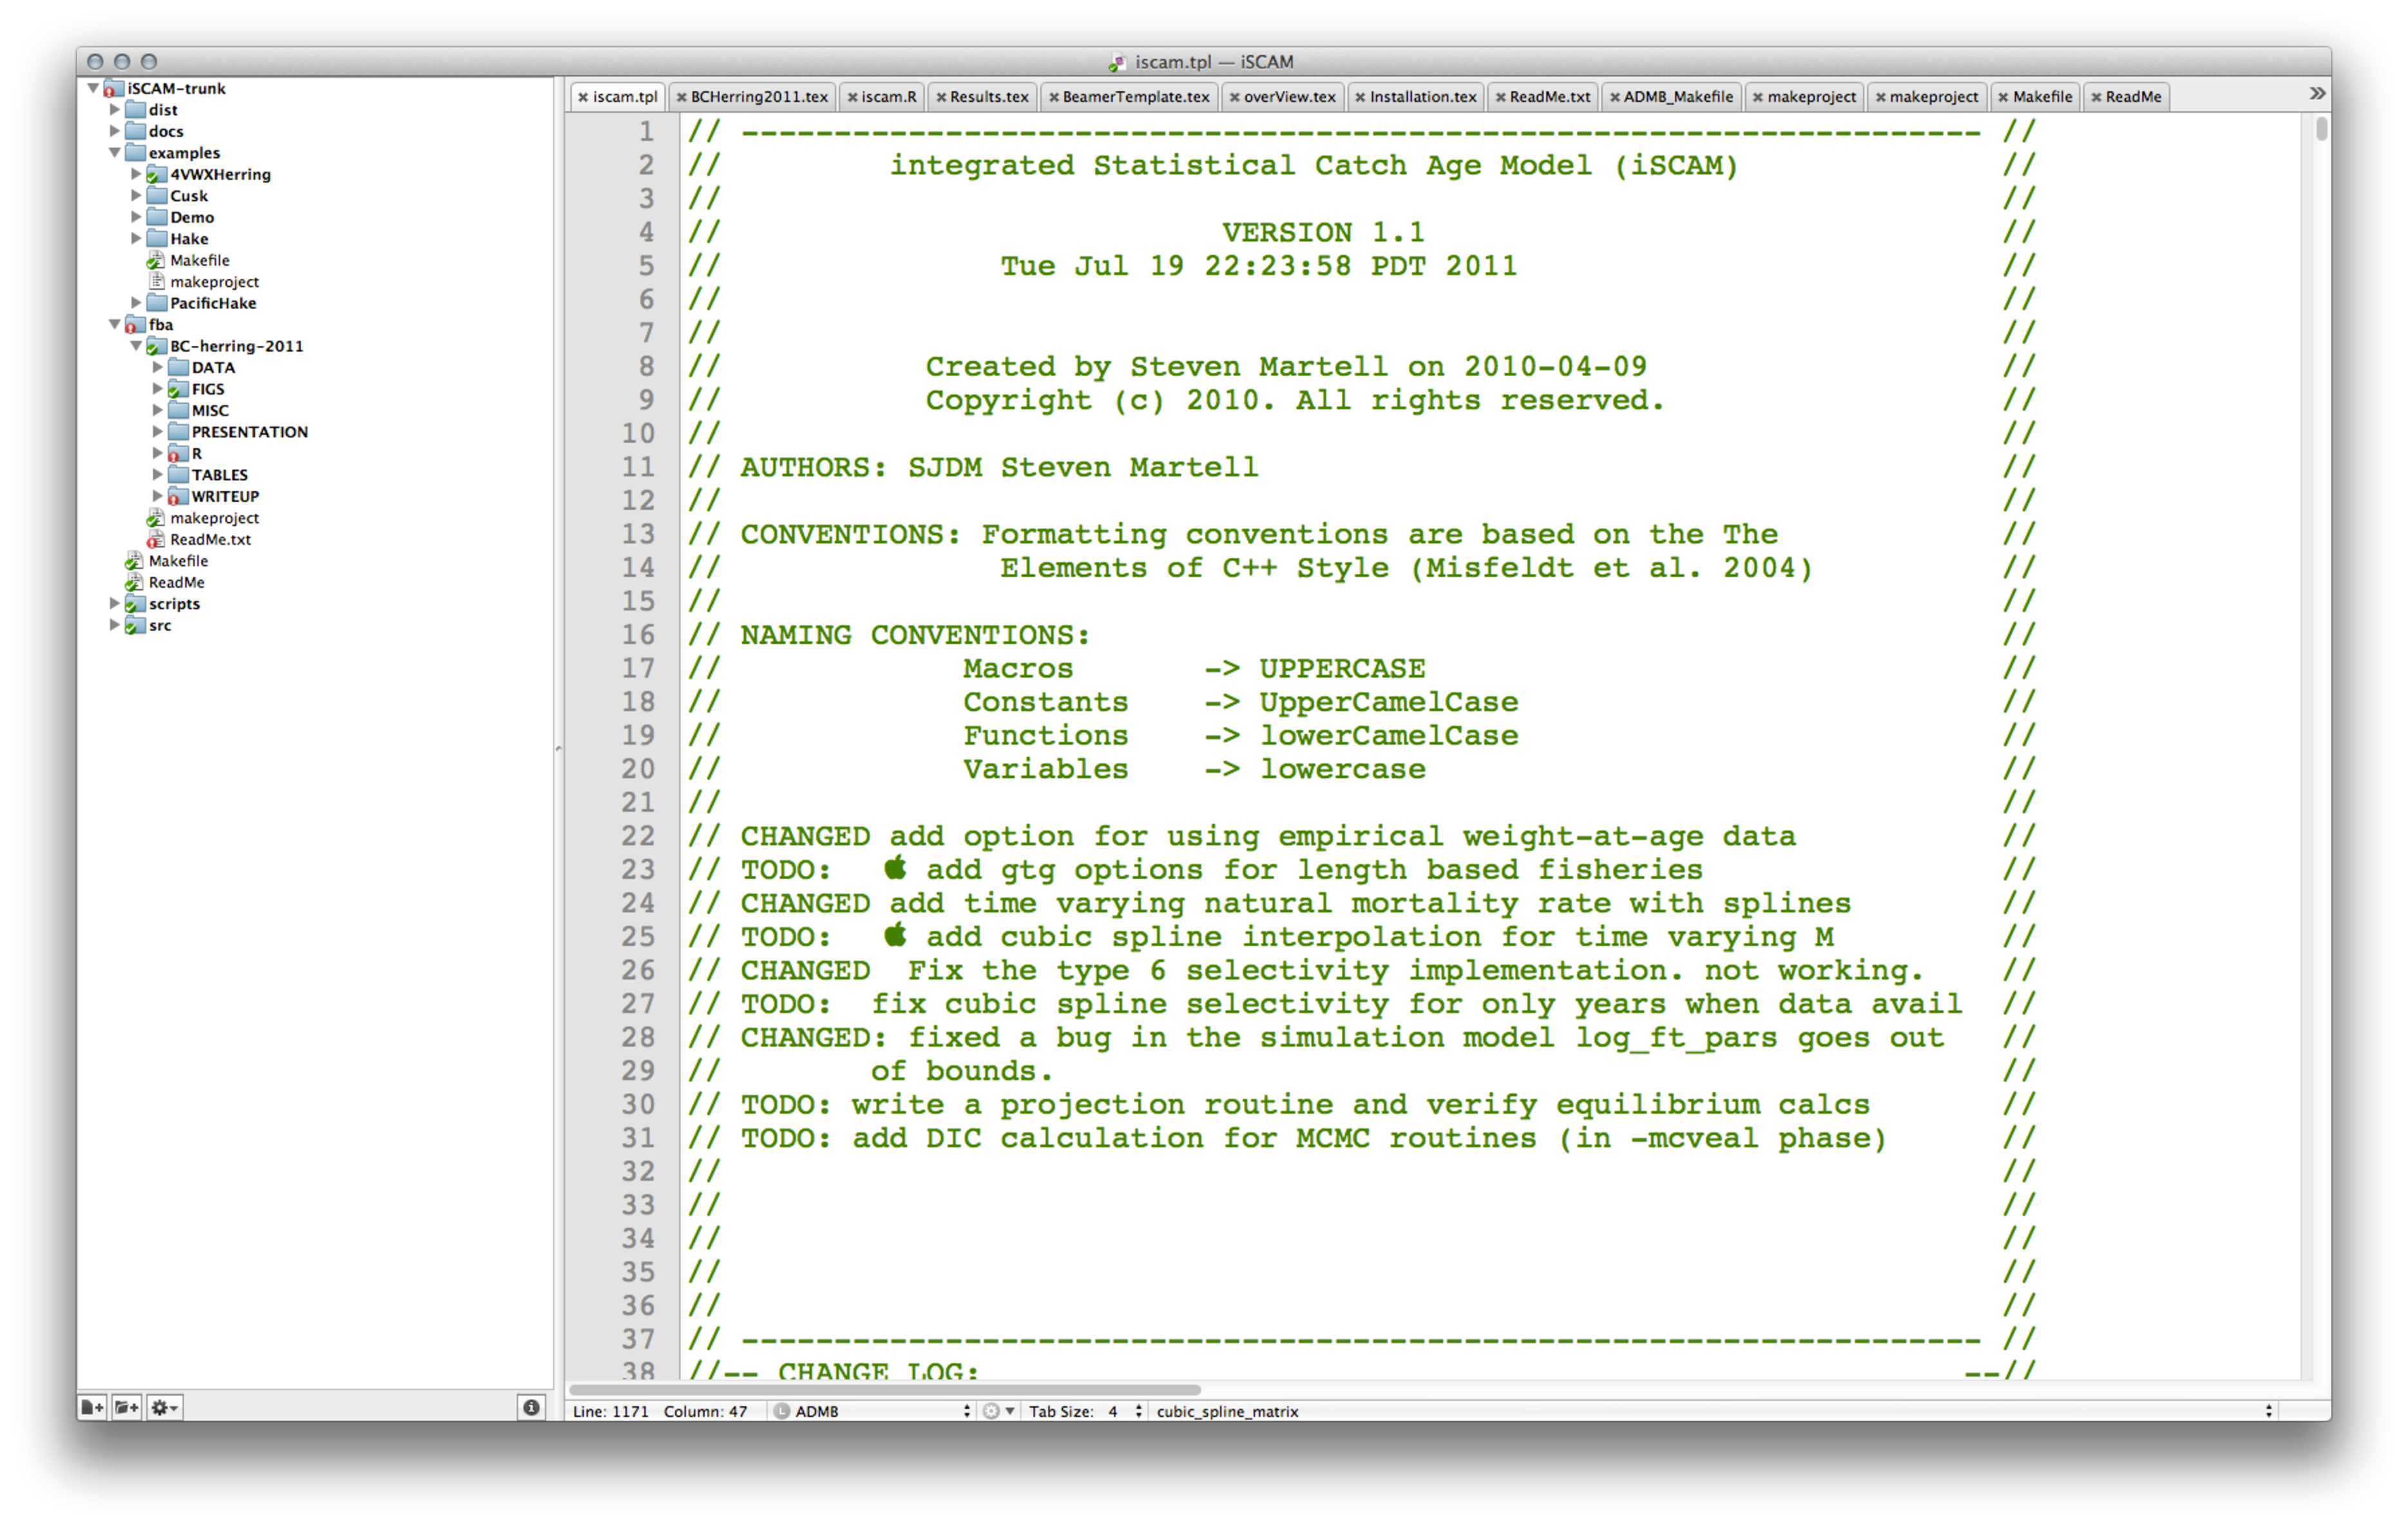
\includegraphics[height=2.5in]{screenCaptures/TextMate.pdf}
		\caption{Textmate on Mac OSX}
		\label{fig:screenCaptures_TextMate}
	\end{figure}
	}
\end{frame}
% subsection text_editors (end)

% section installation (end)